
\chapter{Documents}

\section{Information Sheets}
\label{app:infoSheets}

\textit{The following is representative of the content on information sheets given to participants. The content varied slightly with each study, according to the purposes and processes of the study, as well as if consent was needed from an adult participant or by the guardian of a participating child. The contents below have been edited to maintain anonymity.}

\vspace{10mm}

Dear Sir/Madam,  

\vspace{5mm}

We would like to invite your child or a child you care for to participate in a research project, OurPlace, being run by Open Lab, Newcastle University. 

\vspace{5mm}

\textbf{What is this study about? }

The aim of the research is to explore how digital technologies can support the use of local heritage sites and their surrounding communities as an infrastructure for learning. Encouraging outdoor learning within schools has become a high priority for Ofsted and these sites and communities are often overlooked as teaching resources. Many of these sites – such as parks – have also seen severe budget cuts over the last several years, and through projects like this we hope to increase their perceived value within local communities. 

We are developing a mobile application – OurPlace – which supports the creation and use of playful learning activities in these locations, for use by teachers, families and local community experts. 

\vspace{5mm}

\textbf{What would participation involve? }

This session will involve children and their teachers and assistants using the OurPlace mobile application in [redacted]. This will take place during a normal visit to the park, meaning no additional teaching time will be taken up by the research. 

The children will be asked to complete various activities using the app. These activities have been created by teachers from the school, and have been designed to take advantage of the park environment as a learning resource. Using the app, children may be asked to take photos, record video, draw pictures and plot locations on maps. The materials that the children create can later be used in follow-up classroom activities. The children’s usage and impressions of the application will be used to assess it and shape its development going forward. These impressions may be audio recorded and transcribed for later reference. 

Attached is a consent form, with multiple elements for you to confirm. If you are not comfortable with any of them, feel free to not tick them. The researchers will not take photos of your child without your consent, nor will they collect any information that could be used to identify them. Any images which the children take will be accessible by their teacher.  

\vspace{5mm}

\textbf{What happens if I change my mind during the study?}

It is up to you whether you want your child to take part. You can choose to withdraw your child at any time if you no longer wish for him or her to take part, even after the study has finished.  

\vspace{5mm}

\textbf{Confidentiality} 

All of the data items collected, including photos, audio recordings and transcripts, will be anonymised and stored securely. Only members of the research team will have access to them. Our findings will be published in written reports that will not identify your child or show that they have taken part. If photos taken by the researchers or by children using the application show other children, we will blur out their faces when used in publications or publicity material.  

\vspace{5mm}

We would be grateful if you could complete the attached consent form and return it to your child’s teacher prior to the school trip. 

\vspace{5mm}

Thank you for your time and consideration.   

\vspace{5mm}

Sincerely, 

Dan and Ahmed 

\vspace{5mm}

Contact Details:

Dan Richardson: d.richardson@newcastle.ac.uk 

Ahmed Kharrufa (Supervisor): ahmed.kharrufa@newcastle.ac.uk 

\newpage
\section{Consent Forms}
\label{app:consentForms}

\textit{The following is representative of the content on consent forms given to participants. The content varied slightly with each study, according to if consent was needed from an adult participant or by the guardian of a participating child.}

\vspace{5mm}

\textbf{Parents' Consent Form -- OurPlace}

\vspace{5mm}

{ \RaggedRight
\begin{tabularx}{\linewidth}{ | X | p{30mm} |} 
 \hline
  & Please tick if you agree \\ 
  \hline
 I have had the purpose of this study explained to me. &  \\ 
 \hline
 I have had the opportunity to ask questions about the project and my child’s participation. &  \\ 
 \hline
 I understand that my child does not have to take part. His/her participation is voluntary and can withdraw from this study at any time. & \\
 \hline
 I allow the researchers to take photographs of my child partaking in the study. I understand that any photographs of participants will be stored securely, and will be censored of any identifiable features if published. & \\
 \hline
 I agree to audio recordings being made of my child’s impressions of the application. I understand that these recordings will be transcribed, and any personal details will be removed. & \\
 \hline
 I agree to the use of unnamed quotes in future publications of this work and I understand that any subsequent publication of this research will not identify my child or me by name.   & \\
  \hline
I understand that I can contact the researchers at any time and I have been told how to do this. & \\
  \hline
I understand that any personal data that my child and I provide will be retained and processed by the researcher in accordance with the General Data Protection Regulation (GDPR, 2018). & \\
  \hline
I consent to my child’s participation in this study.  & \\
 \hline
\end{tabularx}
}

\vspace{5mm}

Name (Participant) \rule{5cm}{0.15mm}

Signed (Parent/Guardian) \rule{5cm}{0.15mm}

Signed (Researcher) \rule{3cm}{0.15mm} Date \rule{2cm}{0.15mm}

\newpage

\section{Additional Community OurPlace Engagements}
\label{app:cutcommunityengagements}

\textit{Discussion of these studies was cut from the main document, however I believe them worthy of inclusion here as they either informed changes to the OurPlace application, added to my understanding of the stakeholders who wanted to use it, or provided examples of real-world use cases of the application. }

\subsection{Railway Museum}
\label{app:railwaymuseum}

Designed to transport coals from the region's pits, this site features one of the world's earliest modern railways. As well as the railway lines and several restored locomotives, it boasts a small museum, with a gift shop and tearoom, ran largely by volunteers. One of the site's staff (HP1) was a Heritage Forum member, and wanted to create a walking trail around the site using the OurPlace app.

Initially, HP1 wanted to create a `premium' OurPlace Activity to coincide with a major regional event, which was expected to attract a large number of tourists into the area. The museum had been given access to some funding to take part in the event, and they wished to commission the creation of premium assets to be used in an OurPlace trail. This included audio interviews from local stakeholders, photos from the site and cartoons relating to the site's history. However, HP1 seemed to have a misunderstanding of how the app actually worked: rather than Activities being structured sets of Tasks into which you put content, they thought it was something more akin to a fully customisable website, where creators could change how the app looked and behaved. This confusion, which seemed to stem from the participant's lack of experience with the app and low technical literacy, resulted in the Activity not being made in time for the event.

However, once this confusion had been cleared up, HP1 realised that creating OurPlace content was also less technically demanding than they had originally thought. As they were still uncomfortable with creating an Activity independently, I agreed to assist in making it with them on their iPad device. This resulted in a digitised version of a previously existing trail, using \textit{Location Hunt} Tasks to guide the user between points of interest. Each point of interest had an \textit{Information} Task associated with it, featuring some written information about the location's history and some historical photos. The Activity was made public, and made available to launch from QR codes within the site's museum or by its association with the site's location in the OurPlace app.

\subsection{Lighthouse}
\label{app:lighthouse}

Operated by the local Council, this lighthouse is a local tourist attraction, offering a gift shop, nature reserve and paid entry into the lighthouse itself. This Activity's existence was a particular surprise, as I found it by coincidence while visiting the lighthouse. Having attended the heritage workshop, the lighthouse's staff had soon afterwards independently downloaded OurPlace and created their own Activity for visitors to use. Rather than focus on the lighthouse's history, the creators seemed to be more interested in creating an entertaining activity for visitors: consisting entirely of \textit{Photo Match} Tasks, this Activity simply challenged its users to explore the lighthouse, and find particular features within the space.

\begin{figure*}
  \centering
  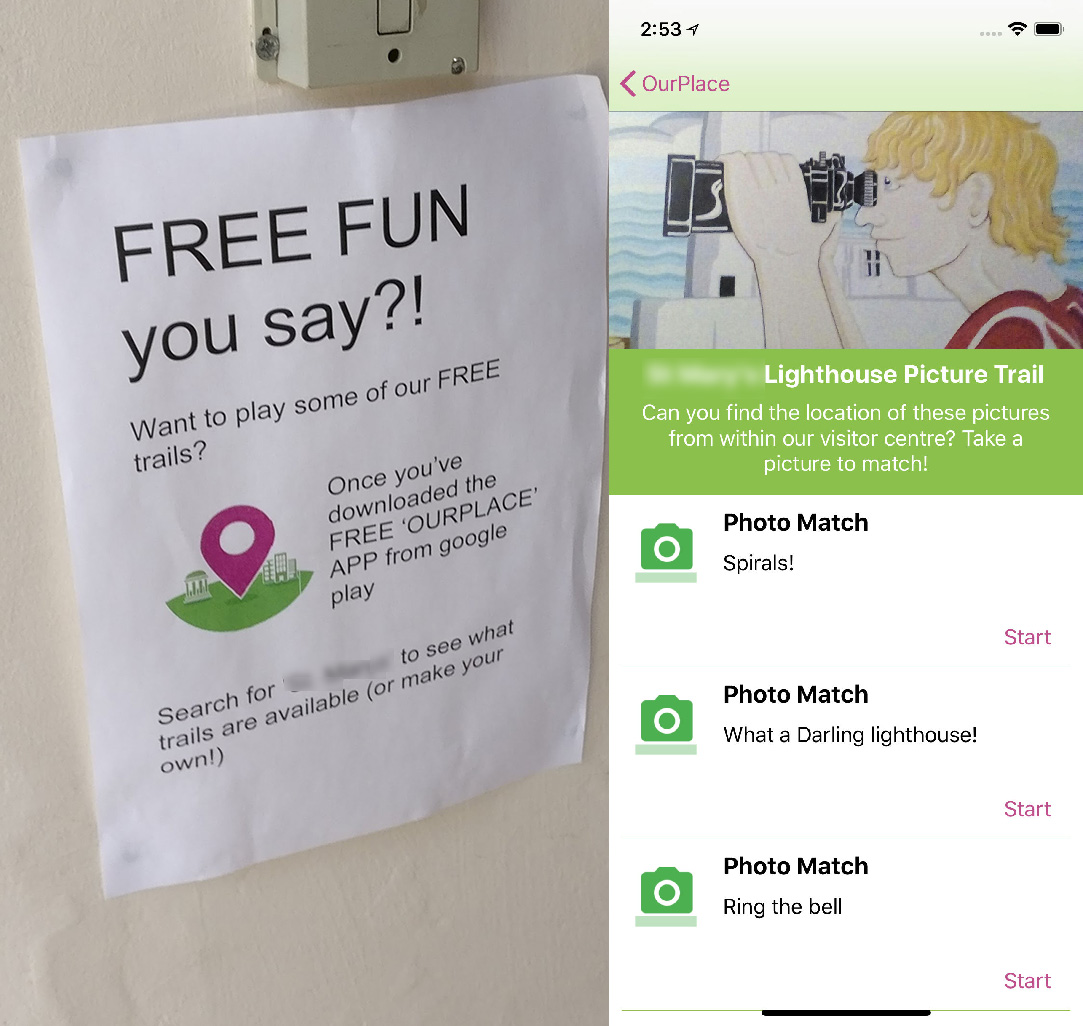
\includegraphics[width=0.65\columnwidth]{images/chapter06/OurPlaceLighthouse.jpg}
  \caption[An OurPlace Activity at a lighthouse]{The management of a lighthouse visitor centre advertise their OurPlace Activity, and invite visitors to make their own.}~\label{fig:OurPlaceLighthouse}
\end{figure*}

The Activity's creators went as far as to create their own poster, advertising the existence of the Activity and featuring the OurPlace branding (Figure \ref{fig:OurPlaceLighthouse}). However, they clearly misinterpreted the app's Activity discovery system: the poster tells users to search for the lighthouse's name, rather than the Activity's share code. The creator also either didn't know about the QR code scanning feature or the app's website, as the poster also doesn't feature the Activity's QR code. 

One interesting thing to note is the poster's call to action, suggesting that visitors create their own Activities around the lighthouse. While some other groups had been hesitant about the idea of anyone being able to create Activities in their space, the lighthouse creator seemed to welcome public contributions and collaboration.

\subsection{Community Railway Partnership}
\label{app:crp}

Another member of the Heritage Forum (HP4) got in touch to enquire about their potential use of OurPlace within their group's educational activities. HP3 was an officer in a `community rail partnership' (CRP) group---a not for profit company that works with train operating companies to `promote, strengthen and protect' the role of a particular railway line in the North of England. The group aims to increase public awareness of the rail services, increase community involvement in the rail lines and strengthen links between the railway industry and the communities and businesses it serves.

HP4 arranged to meet me at Open Lab, along with the CRP's Company Secretary and their Director of Finance, as well as the Community and Sustainability Manager for the railway line's train operating company (HP4 invited this person as they wanted them `\textit{to see that OurPlace could be a great community engagement tool for the Community Rail Partnerships in the North East}', but unfortunately they could not attend the meeting). The group were interested in how they could use mobile learning as a part of their delivery of educational activities on and around the railway. During the meeting I gave a demonstration of the OurPlace app by showing some example Activities (made by both adult stakeholders and school students, covered in Chapter \ref{chap:student-created}), and the process of creating new ones. When conversation moved onto how children themselves could create Activities as a part of the educational events, I also demonstrated the jigsaw activity for creating paper prototypes of OurPlace Activities.

The group brainstormed several ideas about how they could use the OurPlace application to deliver engagements. Ideas included: i) creating Activities in the app which could be completed by visitors and children, both during train journeys and about particular stations (e.g. related to the history of stations and the railway---how they had been used, and how communities had formed around them); ii) children researching these and other subjects, and then creating their own Activities to share with peers and other railway users; iii) using OurPlace Activities as engagement platforms, through which communities could use different Task Types (e.g. \textit{Take a Photo},\textit{ Map Marking}) to engage with the CRP staff---e.g. providing evidence of volunteer work, or report issues with facilities. 

By the end of the meeting, the CRP group had decided that they wanted to use OurPlace as a major part of their engagement programme. The final portion of the meeting was consisted of them discussing the practicalities of what was needed to do so. For example, HP4 saw value in the jigsaw activity as a process for designing Activities (particularly with school groups), and was curious about how they could be made (to the extent that they asked if they could order kits for purchase from Open Lab). The other main considerations were device availability (tablets would have to be bought for the purpose of running OurPlace engagements), and the need to have staff who were i) trained in the use of the OurPlace platform ii) able to dedicate time to design, create and deliver educational sessions which made use of the application.

The group decided that they would apply for a number of grants from the train operating company, both in order to cover the costs of purchasing a number of tablets and to finance a member of staff who would be dedicated to designing and delivering OurPlace engagements for the CRP. At the time of writing, £17,000 of funding has been secured for this, with the CRP having received the funds and starting the process of advertising the role. Unfortunately, this has also been delayed by the coronavirus epidemic.

\subsection{Modern Art Trail}
\label{app:ModernArtTrail}

I was contacted by a retired art teacher (HP2), who had recently started volunteering to run tours of the modern art pieces installed in a local park. They had found out about OurPlace through the Talking Statue installation, and wanted to know how suitable the app would be for use as part of their art trail. After discussing the app and going around the trail, HP2 decided to go ahead with creating an Activity. However, as they didn't own a smartphone and weren't very comfortable with using digital technologies independently, they arranged a follow-up meeting for other members of the park's \textit{Friends} group to attend.

\begin{figure*}
  \centering
  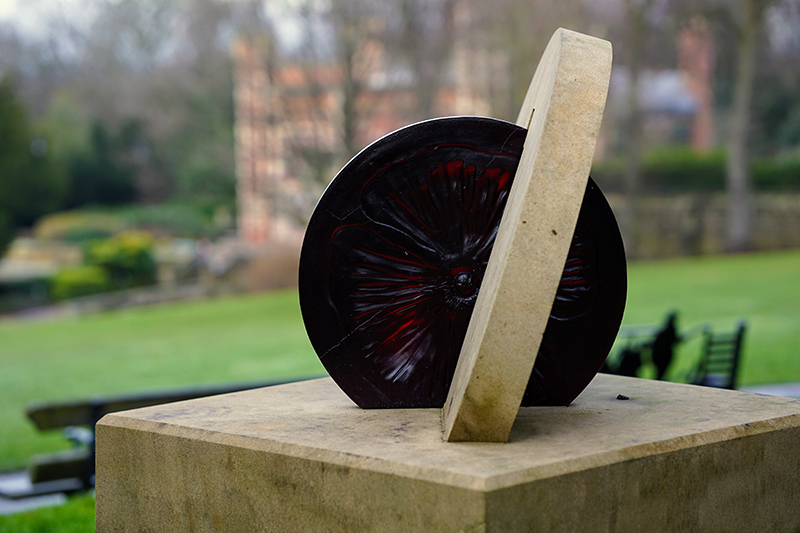
\includegraphics[width=0.7\columnwidth]{images/chapter06/artpiece.jpg}
  \caption[An art piece which was used in an OurPlace Task]{Users of the art trail Activity were challenged to catch the sun's light through this glass poppy, and reflect on how the piece would be altered by different light conditions.}~\label{fig:ParkArt}
\end{figure*}

This meeting took place in a function room in one of the park's main buildings. To assist the group in designing the OurPlace Activity, I took along a jigsaw kit (described in Section \ref{sec:PrototypeWorkshop}) so that they could start designing a paper prototype of the Activity without having to be completely comfortable with the digital interface. After a brief demonstration of the app, the participants started outlining and discussing an Activity using the jigsaw and HP2's notes about the different art pieces, which included blurbs about the artists and the reported meanings of the pieces themselves. 

\begin{figure*}
  \centering
  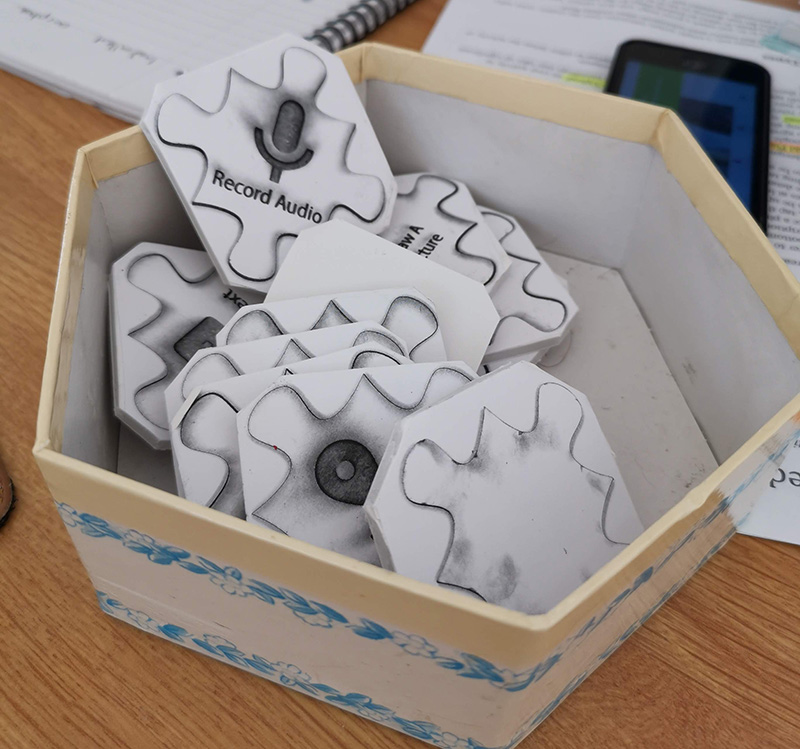
\includegraphics[width=0.65\columnwidth]{images/chapter06/DIY_jigsaws.jpg}
  \caption[Homemade jigsaw pieces created by a \textit{Friends} of the park group member.]{The homemade version of the jigsaw Task Type pieces, created by a member of the park's \textit{Friends} group to assist in designing Activities in the park.}~\label{fig:DIYJigsaw}
\end{figure*}

Rather than be a simple trail which passively delivers information at each stop, the group were interested in how they could use the different functions of the app to enhance the visitor's experiences with the artwork. For example, suggested Tasks included challenging the user to \textit{Take a Photo} of the sun's light passing through the glass of a particular sculpture (Figure \ref{fig:ParkArt}), and then \textit{Record Audio} reflecting on how they think the mood of the piece might change in a different light. Because the trail was becoming so generative, the participants became interested in how they could use people's uploaded responses: ideas included featuring them on the \textit{Friends} group's website, and creating collages of the uploaded images. Because of this, the group were keen on creating the Activity on their own devices, so that they could view authorised responses on the website. They were also concerned about the privacy settings for those who responded, but were satisfied with how the app handles privacy settings once they were clarified.

Rather than create the Activity there and then, the group decided that they wanted to take their time designing the Activity over several sessions, and were happy to do so independently. They claimed to find the jigsaw extremely helpful, and borrowed it to use in their design sessions. Having been able to get used to the structure of the app's Activities through the jigsaw, HP2 now felt more comfortable with the idea of engaging with the technology, and ordered their first smartphone so that they could work on the Activity at home.

Despite this added confidence, they still ran into a couple of issues with the application and asked for help through a follow-up meeting (it turned out they had mixed up the \textit{Record Audio} and \textit{Listen to Audio} Task Types, and were confused as to how they could add audio files while creating \textit{Record Audio} Tasks). During this meeting, one of the members (HP3) revealed that they had created their own Task Type tokens by printing out images of the jigsaw pieces onto foamex board (Figure \ref{fig:DIYJigsaw}), and had been using them to further help them keep track of what Tasks they were creating for each Activity. While we created an Activity together on one of their own phones, HP3 laid these tokens out during the planning stage, and then flipped them over as the Tasks were created. In this way, the tokens acted as a simpler version of the jigsaw, as they didn't require the planning of the Task descriptions.

During this follow-up meeting, HP3 also noted that they had decided to create two versions of their trail: one for the visitors who would normally consider going on the trail anyway, and another version designed for use with schools. While the first one would largely be a digitised version of the existing trail's format, focused on the delivery of information (with some added interactions to stimulate reflection on the art pieces), the version designed for schools would make use of the seamless nature of the OurPlace application. This version would focus on the more creative and generative Task Types, with the explicit intention for students to generate materials and record their reflections in-situ for later use upon return to the classroom. When I enquired what had inspired them to use the app in this way, HP3 revealed that they had printed and been thoroughly (with the liberal use of highlighter) reading one of the project's resulting publications \citep{Richardson2018} of their own volition. Unfortunately this study was interrupted from progressing further by the COVID-19 epidemic, and the trail has not been completed as of the time of writing.

\subsection{Heritage Forum Conference, OurPlace Workshop}
\label{app:HeritageOurPlaceWorkshop}

I also held a short workshop at the Heritage Forum's conference the following year. This workshop consisted of a short presentation introducing the project, and then an interactive section in which participants were able to try out the OurPlace app for themselves. Following a tour from the conference venue's manager, I pre-prepared an Activity about the building and loaded it onto the available tablets. The Activity was designed to show how the app could be used both as a form of digital interpretation and as way to provide visitors with a more interactive experience. As the Activity was limited to being inside the venue, I chose not to use \textit{Location Hunt} Tasks. Instead, the Activity guided the participants around to different areas of the building to find various QR codes, which when scanned revealed information about its heritage and various interactions as Follow-Up Tasks.

While short, this workshop highlighted how varied the levels of digital literacy can be, even amongst people of similar demographics. For example, a representative from one heritage group was interested in if they could run their own version of the OurPlace server, offline on their local network---their site was a cave system, and didn't have access to the Internet. This person clearly had technical knowledge, as they were asking about how they could use the open-source nature of OurPlace to make it more suitable to their own circumstances. However, in the same workshop were multiple individuals who had never used an app, or seemingly even held a smart device before. It was clear that I had over-estimated the base technical literacy of the participant group, as this person was asking me to explain what a smartphone app was---while the app's documentation had explained some basic information for non-technical users (e.g. how to download the app from Google Play), it was within with an assumed base level of knowledge about the \textit{existence} of the technologies and interface metaphors the app is built upon. Accommodating both of these potential audiences was extremely difficult in the workshop, but it was clear that the many of audiences that the app was targeting (i.e. heritage enthusiasts, institutions and volunteer groups) would also be comprised of individuals with a similar mix of degrees of comfort when dealing with technology.

\section{Additional Teacher engagement: Petting Zoo Trip}
\label{app:pettingzoo}

\textit{Discussion of this study was cut from the main document, however I believe it still worthy of inclusion here as it informed changes to the OurPlace application}

Shortly after the first trip with Teacher 1, I led a one-off engagement with a different school's reception class (N=28, ages 4-5) and their teacher. While the previously discussed study was primarily investigating how the approaches taken by the teachers towards the application changed over time, this one was much more focused on immediate results: exploring new ways of using the ParkLearn platform, observations of interactions with the different Task Types, and testing it for bugs. 

Following the same methodology as the initial engagements with Teachers 1 and 2, the teacher was introduced to the application separate to the class during an hour-long meeting, using example Activities to demonstrate the app's functionality. The latter half of the meeting consisted of the teacher creating an Activity for the class's trip to a park and petting zoo the following week. This Activity consisted of 5 different Tasks and Task Types: `What minibeasts can you find?' (\textit{Take Photos}), `Draw what you can see from the bridge!' (\textit{Draw a Picture}), `Can you find the petting zoo?' (\textit{Location Hunt}), `Record your favourite animal that you can see!' (\textit{Record Video}), `Record your friend making their favorite animal noise!' (\textit{Record Audio}). As this school was reliant on me for access to tablets, this limited the number of devices to twenty between the students---meaning several children had to share one between two. My observations and the verbal impressions from the children made during the trip were recorded as field notes. The practical nature of these notes meant they could directly inform the development of the application, without needing to undergo thematic analysis.

In total, the children created and uploaded 19 responses to the Activity, consisting of 106 photos, 12 drawings, 14 videos and 8 audio recordings. Despite being extremely young, the children proved to be able to use the application effectively, especially when completing camera-based Tasks. They particularly enjoyed the \textit{Location Hunt} Task Type, thanks to both the audiovisual component of the increasing speed of the animation and beeping, and the exciting ambiguity of not knowing exactly where the Task will take them. However, there were some elements of this early version of ParkLearn which frustrated the children. For example, this version only allowed one drawing, video, or audio recording to be made in response to a Task---if another one was produced, the first would be overwritten. This decision had been made with the intention of simplifying the interface (not having multiple responses listed for each Task) and reducing the amount of storage and bandwidth required when uploading responses. However, during this study it led to children overwriting their work by accident, or being frustrated at not being able to produce multiple responses to a given Task. As a result, later versions of the application introduced the ability to produce multiple pieces of media to a given Task.

\section{Thematic Analysis Example}
\label{app:analysisexample}

\begin{figure*}
  \centering
  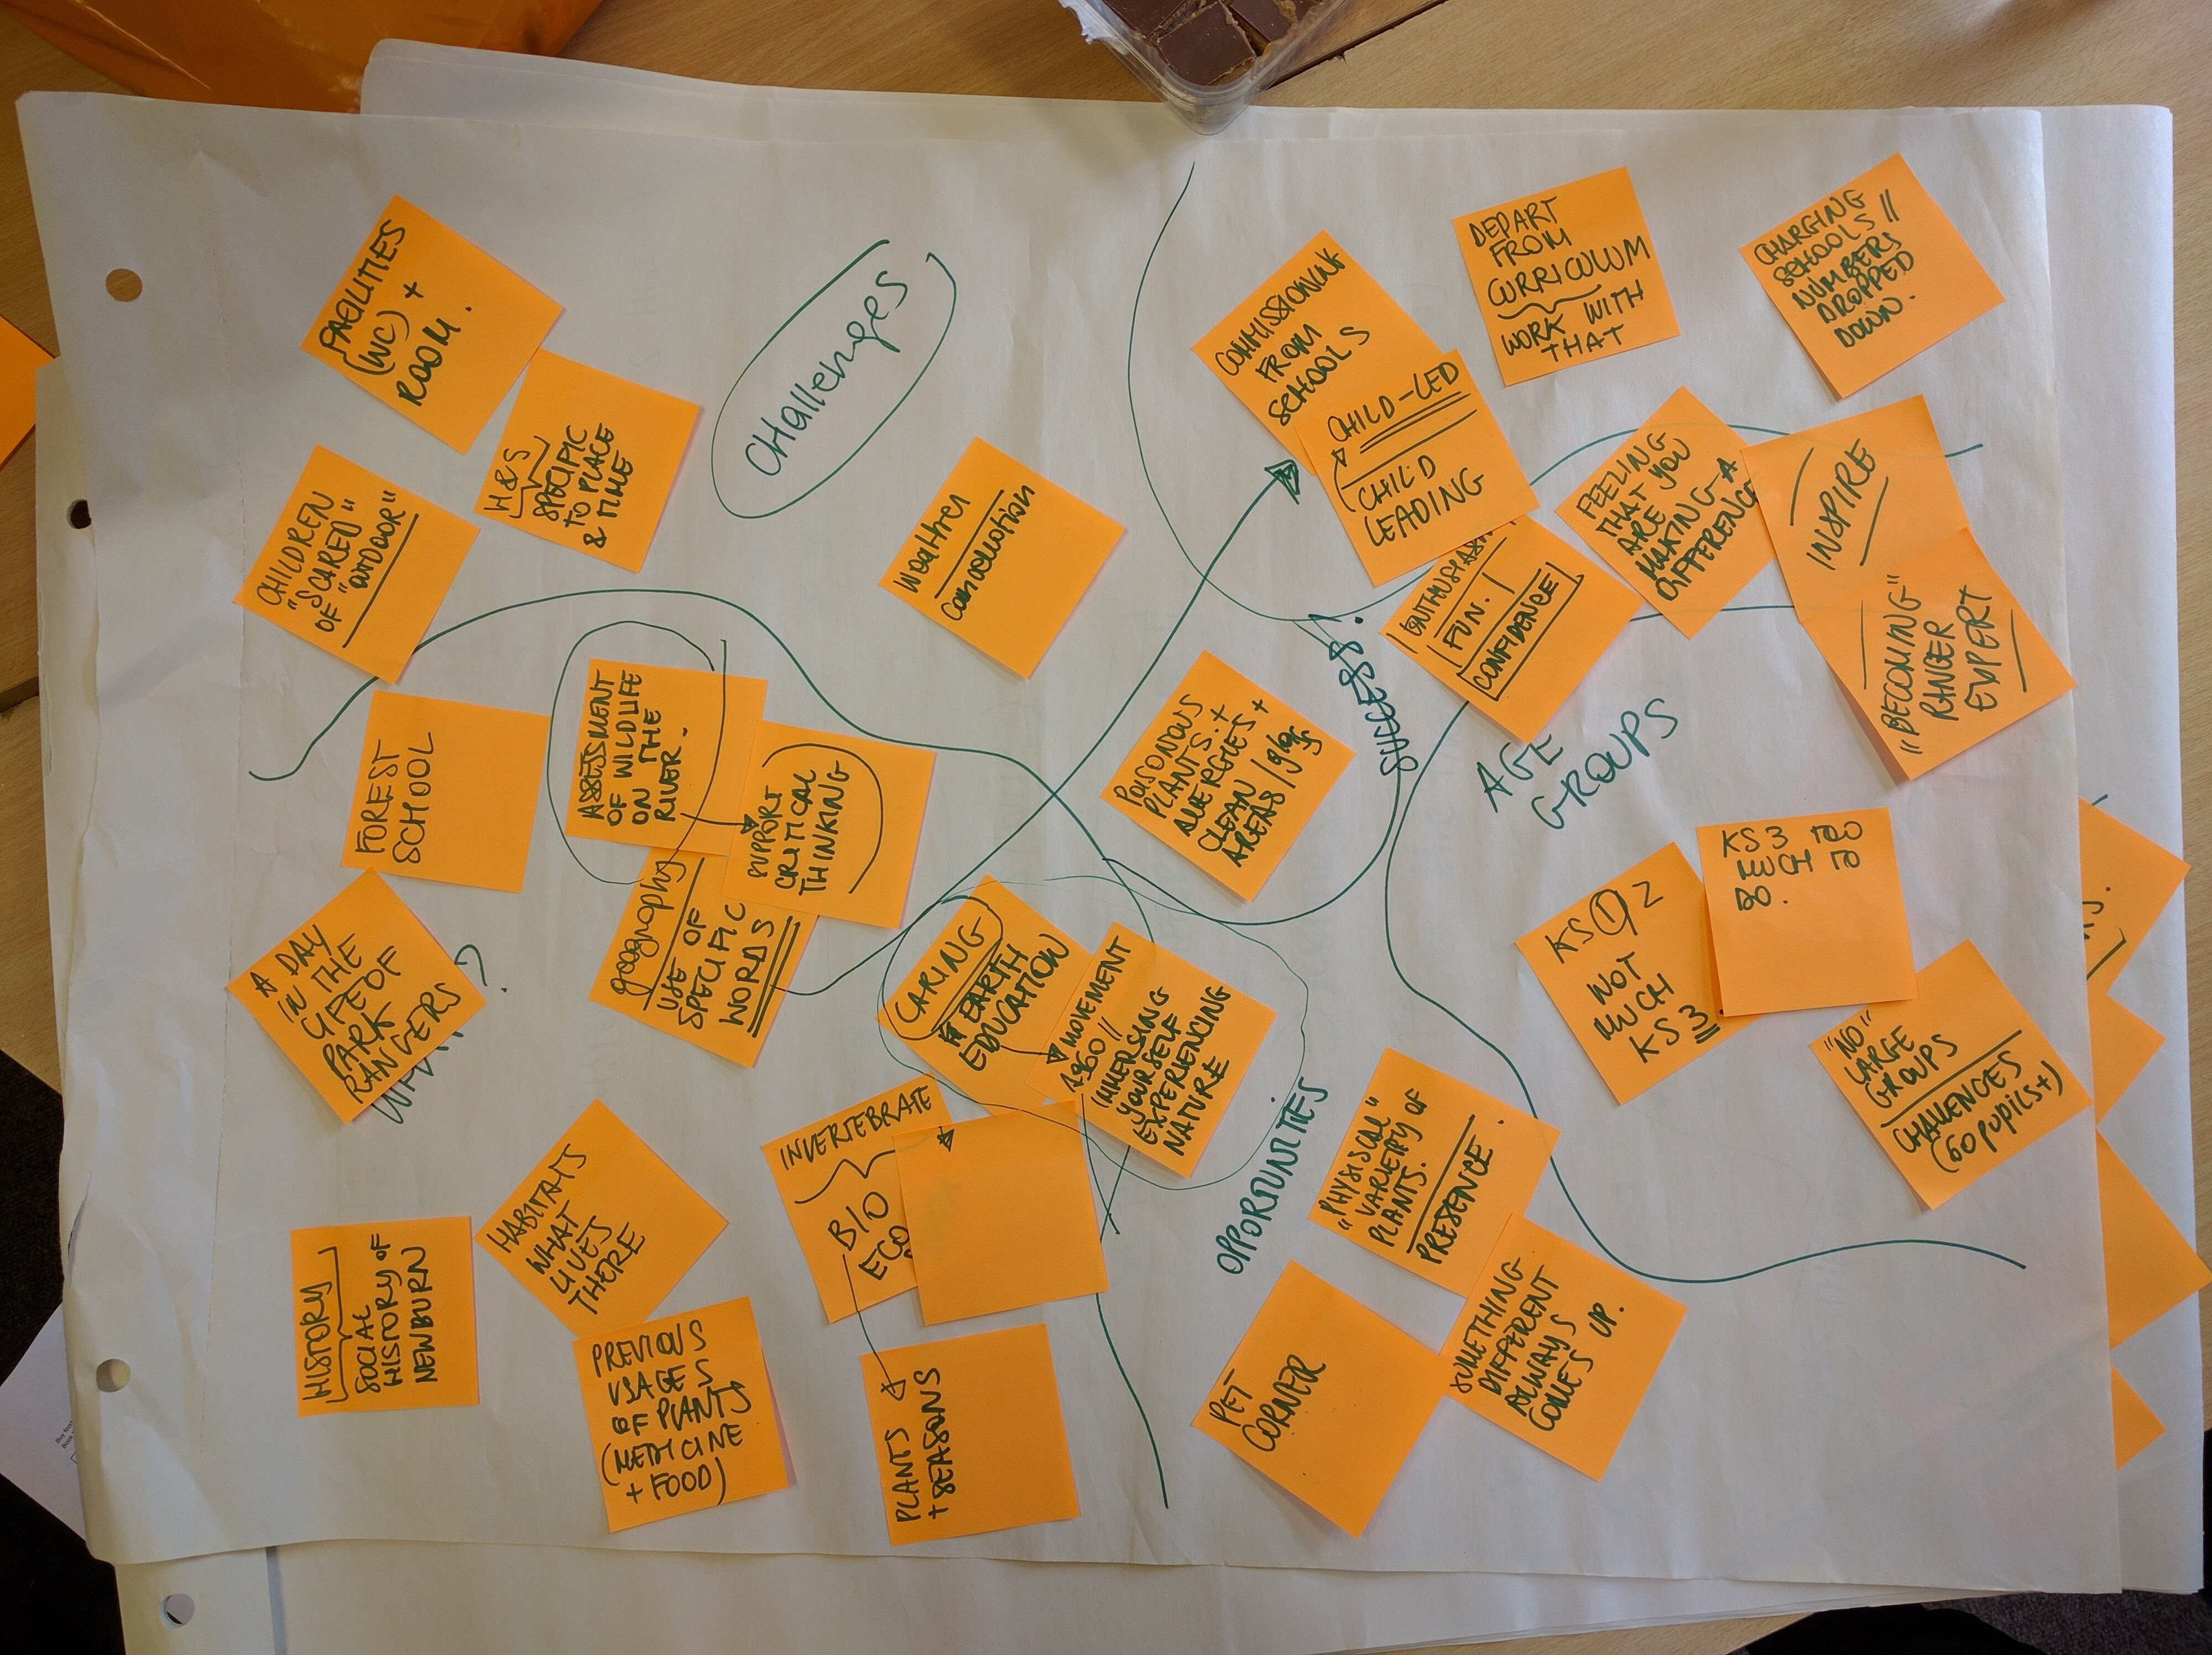
\includegraphics[width=0.8\columnwidth]{images/appendix/clara.jpg}
  \caption{Example results of a theme triangulation session with Dr Clara Crivellaro}
  \label{app:triangulationexample}
\end{figure*}


\textit{The following is an anonymised example of the contents of a Word document featuring the codes and resulting themes developed from printed transcripts, following the process discussed in section \ref{sec:applyingdbr}. This particular document is the final result of the codes generated from the transcripts of the engagements described in chapter \ref{chap:student-created}. Due to space limitations, the entire transcripts cannot be included. Themes are presented in bold, with each theme's codes then presented in italics, and anonymised pertinent quotes and observations for that code included in regular text.}

\vspace{5mm}

\textbf{Students’ Desire for Independence}

\par\noindent\rule{\textwidth}{1pt}

\textit{Children eager to contribute, have responsibility, grow up}

\par\noindent\rule{\textwidth}{1pt}

- [researcher] “The children help out a lot then. So if you guys were show children, you’d be helping work. Does that sound good? Would you want to be working?” \\
- [children] “Yes!”\\
- [researcher] “Why would you want to be working?”\\
- [child1] “To get money to support my family”\\
- [researcher] “To get money, help your family get money yeah.”\\
- [child2] “To provide for your family and buy a house and if you have some money left over to buy a car”

{\centering
  \noindent\rule{0.5\textwidth}{0.4pt}\par
}

- [child7] “If you’re doing the same as your family, if you’re a child you might not get paid as much because people could want to only go to adults and think that children are not responsible yet.”  

\par\noindent\rule{\textwidth}{1pt}

\textit{Doesn’t want to be restrained by an inherited job}

\par\noindent\rule{\textwidth}{1pt}

- [child1] “The reason that I wouldn’t like a job like your parents is that for example, at the hoppings you just go around selling for a pound and stuff, and you only get a pound. For example, say if I was an engineer, I would get for example 20 or 10 pound. It’s more, I get paid more. If I did the same as them, I wouldn’t want to do that - wait around, and maybe they wouldn’t even come, have a ride. It’s like more better, more educational for you. Saying, ‘You want a ride?’ is not really, like useful for people. Being a mechanic is more hard, and if you just carried on a tradition you might not really like it, like what they’re doing.”\\

{\centering
  \noindent\rule{0.5\textwidth}{0.4pt}\par
}

- [researcher] “Would anyone here be unhappy if they had to do what their parents did? Does anyone want to do something different to their parents?”\\
- [children] “Yeah”\\
- [child8] “It’s just natural”\\
- [child2] “It’s natural to do something different”\\
- [researcher] “That might not be true, you get people who do the same jobs as their parents and pass it down for generations”\\
- [child9] “I don’t want to do my parents’ job”\\
- [child10] “I don’t want to do my parents’ job because my Mam doesn’t work and my Dad works as a builder”\\

\par\noindent\rule{\textwidth}{1pt}

\textit{Children’s prepped questions for showchildren focusing on them earning money and their role/impact}

\par\noindent\rule{\textwidth}{1pt}

- [child2] “How much do they make in a week?”\\
- [child14] “How much money do you earn?”\\
- [child18] “How much money do you make in a year”\\
- [child20] “What’s your net worth”\\
- [child21] “Do you enjoy it and do you get enough money?\\
- [child27] “Have you ever designed a ride”\\
- [child28] “Have you ever chosen a ride to build”\\
- [child1] “I would ask them their age, then I would ask an eleven year old, have you made something yet. And I would ask a seven year old, have you made a little model.”

\par\noindent\rule{\textwidth}{1pt}

\textit{Expectations of financial knowledge, independence and respect within the family}

\par\noindent\rule{\textwidth}{1pt}

- [researcher] “Do you think the kids would know what? Do you think they would know how much money is coming in for the family?”\\
- [children] “Yeah”\\
- [researcher] “Why do you think that? How do you think they’d know?”\\
- [child1] “They’re good at maths”\\
- [child2] “Their grandparents would tell them”

\par\noindent\rule{\textwidth}{1pt}

\textit{Students earned independence, teachers’ trust, through maturity}

\par\noindent\rule{\textwidth}{1pt}

- [teacher] "What I enjoyed was trusting you to work with Dan and Georgina, because that means you're really Year 4s, doesn't it? That we can trust you to do something, away from the class teacher and still do something really, really good. So well done."

{\centering
  \noindent\rule{0.5\textwidth}{0.4pt}\par
}

- [teacher2] "I would like to also point out how good they were as teachers, as well. They really came into their own. The Year 4s were outstanding, very good, and I was very proud of them."\\ 
- [teacher] "I think you really are stepping up to be Year 4s, it's wonderful to see. Well done all of you, that was brilliant. And if you're very grown up, you get to do very grown up things. So let's give year 4 a clap."


\par\noindent\rule{\textwidth}{1pt}

\textbf{Positive Outcomes of Students’ Independence}

\par\noindent\rule{\textwidth}{1pt}

\textit{Teachers capitalising on students' independence}

\par\noindent\rule{\textwidth}{1pt}

- [teacher2] “That’s why you give them very simple things. But they don’t have to do all of these things”\\
- [teacher1] “Oh no, I just want to know what-”\\
- [teacher2] “The groups will decide what best fits their thing”\\
- [teacher1] “Absolutely. I just want to know what is available.”

{\centering
  \noindent\rule{0.5\textwidth}{0.4pt}\par
}

- [teacher2] “The kids are much better at thinking of ways they can adapt what they've found to other things.”

{\centering
  \noindent\rule{0.5\textwidth}{0.4pt}\par
}

- [teacher2] “It would be quite nice for them all to make a section to collaborate.  Then each group can come up with their own activities, and then put it together a nice big, meaty thing at the end, a tour of Gosforth.”

\par\noindent\rule{\textwidth}{1pt}

\textit{Creating activities involves asking questions -> independently searching for answers}

\par\noindent\rule{\textwidth}{1pt}

- [child1] “We are going to find Newcastle Castle’s roof...and do lots of activities. First, I’m going to ask them to find out when it was made.”\\
- [researcher] “Oh that’s a good question, isn’t it. Do you know the answer?”\\
- [child1] “No. But I can search it up on Google”\\

\par\noindent\rule{\textwidth}{1pt}

\textit{Desire for access outside of school}

\par\noindent\rule{\textwidth}{1pt}

- [child1] “Is this app available on any type of tablet, iPad?”\\
- [researcher] “Yeah, you can download it at home if you want to”\\
- [child1] “I tried, it didn’t work”\\
- [researcher] “Did you try recently?”\\
- [child1] “No”\\
- [researcher] “If you try again it might, because I did fix something”

{\centering
  \noindent\rule{0.5\textwidth}{0.4pt}\par
}

- [child1] “Wait... what app is this on?”\\
- [researcher] “It’s called OurPlace, it’s one that I made”\\
- [child1] “Can you get it on iPads?”\\
- [researcher] “Yep”\\
- [child1] “Ah! Can I get the app?”\\
- [researcher] “Yeah, it’s free”\\
- [child1] “Yay!”

\par\noindent\rule{\textwidth}{1pt}

\textit{Tools were generalisable enough to facilitate and capitalise upon students’ varied ideas and approaches}

\par\noindent\rule{\textwidth}{1pt}

- [teacher2] "They were very different as well weren't they? The ideas. Even though you all started off with the same tools."\\
- [teacher] "Well that's what's great--that everybody's had their own ideas"

{\centering
  \noindent\rule{0.5\textwidth}{0.4pt}\par
}

Observation: Used OurPlace as a platform for their own jokes/memes (Celebrate Good Times, prequel memes), putting these to use constructively within school projects

\par\noindent\rule{\textwidth}{1pt}

\textbf{Lack of Scaffolding Leading to Focus on Tech over Content}

\par\noindent\rule{\textwidth}{1pt}

\textit{Left to their own devices without much scaffolding/guidance, Y8 students created very general/vague activities}

\par\noindent\rule{\textwidth}{1pt}

- [researcher] “In terms of making it useful for a trail… ‘an area of interest’ is very general, isn’t it?”\\
- [student] “Yeah, I guess. So instead of saying ‘an area of interest’, give something more specific?”

{\centering
  \noindent\rule{0.5\textwidth}{0.4pt}\par
}

- [teacher] “It might have all the bells and whistles, but if you’re not learning anything it’s pointless.”

{\centering
  \noindent\rule{0.5\textwidth}{0.4pt}\par
}

- [student2] “I think we’ve found it easier than other groups because we focussed more on the content than using all of the different interactions. So a lot of the content can be the same [as the analogue version], it’s just changing how to interact with it”

{\centering
  \noindent\rule{0.5\textwidth}{0.4pt}\par
}

- [teacher] “it seems to me that some of you have got the basics of the technology, I think. I think that there’s some good stuff technology-wise. I think what needs some further thought, is what you’re actually asking them to do in terms of the content.”

{\centering
  \noindent\rule{0.5\textwidth}{0.4pt}\par
}

- [teacher] “You’ll learn from that experience though, won’t you. That was quite a basic set of parameters to work with, wasn’t it? I know that if that had been more freeform and open-ended, that would have been rather worse. So, they had a Whitburn trail which was highly structured, and they had the opportunity to deviate and go as far as they want away from it, within the parameters of making it workable and interesting. I don’t know about you but the thing I was coming across again and again was the lack of challenge, the lack of depth, and the kind of things they were asking was really just playing with the technology rather than [engaging with the history]”

{\centering
  \noindent\rule{0.5\textwidth}{0.4pt}\par
}

- [teacher] “[student]’s looked coherent in terms of the actual structure. But when he was asked about what he was asking them to do, he had no thought.”

{\centering
  \noindent\rule{0.5\textwidth}{0.4pt}\par
}

- [teacher] “It’s worth cogitating about what parameters you probably need to introduce, to guide them towards deeper thinking. I think it’s more of a success for the technology, the medium, than the actual content. It needs to be worth doing, there’s no point in having all of the bells and whistles if there’s no substance.”

{\centering
  \noindent\rule{0.5\textwidth}{0.4pt}\par
}

- [researcher] “Some of them said they found it a bit easier than others did to convert to the pen and paper, because they were less reliant on the app’s features. I don’t know how true that was.”\\
- [teacher] “I think it depends on how they were thinking about the task in the first place - maybe, if they’d been highly creative, obviously they’d struggle, but if they were highly creative and lost their focus, then they’d be miles away. If they were less creative, but focused on the nature of the content they’d probably find it easier to transpose. What we want is something in-between.”

{\centering
  \noindent\rule{0.5\textwidth}{0.4pt}\par
}

Observation: Showchild’s repeated engagement about how to improve his QR code task – wanted to create a richer activity. Implies that the creation session was too short, lacked enough explanation.

\par\noindent\rule{\textwidth}{1pt}

\textbf{Teaching Pressures \& Limitations}

\par\noindent\rule{\textwidth}{1pt}

\textit{Time pressure}

\par\noindent\rule{\textwidth}{1pt}

- [teacher] “It’s just time pressure, isn’t it? I’m trying to meet so many times, it just… numbs you, so busy.”

\par\noindent\rule{\textwidth}{1pt}

\textit{Data privacy issues with new tech platforms + data formats }

\par\noindent\rule{\textwidth}{1pt}

- [teacher] "What about [sharing] kids’ voices – are voices ok? They don’t mention who they are, do they? So it should be. […] I should know, but I don’t. It’s not something we ever come across, you see."

\par\noindent\rule{\textwidth}{1pt}

\textbf{Sharing Activities \& Knowledge with Others}

\par\noindent\rule{\textwidth}{1pt}

- [headteacher] "You really need to listen to what they [Year 4] have to say, because they have designed this themselves. They are your teacher, ok? And I would like Year 4s to tell me if there's anyone not listening to you, ok? Please listen, because they've worked really hard--they've worked two weeks doing this, and they're really excited about you having a go."

\par\noindent\rule{\textwidth}{1pt}

\textit{Self organising groups - younger kids wanted to make sure they got to do all of the activities, were keeping track of which Year 4s they had been with}

\par\noindent\rule{\textwidth}{1pt}

- [teacher] “Which part of it did you enjoy most?”\\
- [student3] “Today, getting to go around and swap with other people and getting to find out about theirs”\\
- [teacher] “So then did that help you, when you had a go at someone else’s, did it make you think ‘oh, we could have done this on our app’, or?\\
- [student3]  “Yeah”\\
- [researcher] “Do you think swapping was quite important? Do you think that made it more interesting?”\\
- [students] “Yes”\\
- [researcher] “Do you think it helped that it was people in your class that you were swapping with? Or if it was another school or something, do you think that would be interesting, if you made stuff for another school, and you used theirs?”\\
- [student7] “I think that if we made stuff for another school that made them learn it would be really good, because you could make it about your school.”\\
- [teacher] “Yeah that would be really interesting. We’ve talked about Mia’s school, she’s out in the countryside where there’s like, ten children in a class. That’s a very different school experience to what you have here, so that would be an interesting thing to do, wouldn’t it? To swap it and see what their daily life is like and what yours is like.”

\par\noindent\rule{\textwidth}{1pt}

\textit{Teachers recognising the value of children exchanging activities and ideas}

\par\noindent\rule{\textwidth}{1pt}

- [teacher] “I think that would have been better, wouldn’t it? If we’d actually done it and then taken a different group of children out to use it, but it’s just time pressure, isn’t it. So I think that if they had then in the final stages gone out with perhaps a partner from another class-so that might have worked. So if you did it with one class, and when they finish, take the other class with them, and they’ve got to show it and not take over. And then they can evaluate: ‘Oh, I should have done this, perhaps if I’d done that it would have been better’-watching the other child do it.”

{\centering
  \noindent\rule{0.5\textwidth}{0.4pt}\par
}

- [teacher] “I run a school for the children [at the fair], so if you want to come and do a project with Showmens’ children, if you want to do a cultural minority, they are cultural minority. […] Their lives are so different, that actually it would be a nice tool to share with other children what it’s like to be a Showman. It’s a totally different way of life. […] And the children would love to do something, because as I say their work packs are super dull.”

\par\noindent\rule{\textwidth}{1pt}

\textit{Children sharing technical knowledge with newcomers}

\par\noindent\rule{\textwidth}{1pt}

- [teacher1] “I’ll know what those 8 [potential topics] will be. It’ll come under the umbrella of the kids get to take ownership of it, because they get to choose what they want to research. But we’ll steer it, so that they do research those things.”\\
- [child3] “How do we do the app?”\\
- [researcher] “Oh! Have you not done it before?”\\
- [child1] “No cos she goes swimming. I’ll help Phoebe”\\
- [researcher] “Are you able to work together on it?”\\
- [child1] “Yeah!”

\par\noindent\rule{\textwidth}{1pt}

\textit{Children identifying the value of sharing their knowledge}

\par\noindent\rule{\textwidth}{1pt}

- [researcher] “How are we doing? ‘How deep is the well?’ That’s a good one.”\\
- [child3] “This is actually helpful, because some people didn’t get to see the well.”\\
- [researcher] “Yeah that’s a good idea. So are you making a quiz to teach them about it?”\\
- [child3] “Yep”

\par\noindent\rule{\textwidth}{1pt}

\textbf{Activity Creation as a PBL End-Product}

\par\noindent\rule{\textwidth}{1pt}

\textit{Ownership and sharing of activities enhancing PBL }

\par\noindent\rule{\textwidth}{1pt}

- [teacher1] “Looking at how to properly analyse photographs, give them frames of reference, things like that. But, in terms of an end goal - I thought this (points at app) would be a nice thing to do.”\\
- [teacher2] “Yeah, that’s how we’d want to do it. Sounds good”\\
- [teacher1] “No it really does. Because we do these lessons just as lessons, but the fact that they now mean something in terms of an end product. It’s not just like, here’s some maps- find out what’s changed. We’re gonna make this app and we’re going to do a hunt, find out what’s changed and find something that you’re going to research. Just makes it that much more meaningful”\\

{\centering
  \noindent\rule{0.5\textwidth}{0.4pt}\par
}

[teacher1] “Making that app will be mint. If you can make it so that they all submit their own activities...that would be fab. I think this will be an amazing project.”

\par\noindent\rule{\textwidth}{1pt}

\textit{Approach supports a variety of learner preferences \& interests}

\par\noindent\rule{\textwidth}{1pt}

- [researcher] "And what was your favourite thing about doing it?"\\
- [child1] "I enjoyed being the teacher."\\
- [child2] "Being outside"\\
- [child3] "I enjoyed making the app itself"

{\centering
  \noindent\rule{0.5\textwidth}{0.4pt}\par
}

Note: School had been warned about its lack of ‘social mobility’, lacking drama and other courses. Teacher noted that engaging with both local communities and researchers had a positive impact
